\documentclass[conference]{IEEEtran}
\IEEEoverridecommandlockouts
% The preceding line is only needed to identify funding in the first footnote. If that is unneeded, please comment it out.
\usepackage{cite}
\usepackage{amsmath,amssymb,amsfonts}
\usepackage{algorithmic}
\usepackage{graphicx}
\usepackage{textcomp}
\usepackage{xcolor}
\usepackage{hyperref}
\usepackage{graphicx}
\usepackage{smartdiagram}

\def\BibTeX{{\rm B\kern-.05em{\sc i\kern-.025em b}\kern-.08em
    T\kern-.1667em\lower.7ex\hbox{E}\kern-.125emX}}
\begin{document}

\title{Hello I'm a title\\
{\footnotesize Network Tour of Data Science Report, January 2019}
}

\author{Isabela Constantin, Ad\'elie Garin, Celia Hacker, Michael Spieler}

\maketitle

\section{Introduction}
Using the Wikipedia data set that is now open source, we would like to understand how the number of views on one page spreads in the linked pages when some unexpected event happens. We chose to study specifically the pages of three famous people who died in the past few years and we are interested in the number of views in the pages that are related to the main page of the person who died. We will consider two times for the number of views: the day before the person dies and the day of the death. 

\medskip

For each person who died, we build a specific graph around their wikipedia page by taking wikipedia pages as nodes and links from one page to another as directed edges. We will use both the directed graph, in which one page which is linked to the other leads to only one direction for the concerned edge, and the undirected graph, for which there exists an edge if and only if there is one page linked to the other. The full construction of the three graphs is described in Section \ref{acquisition}. For each node $i$ (corresponding to a wikipedia page) of a graph, we are interested in the following quotient: \[Q_i:=\frac{\text{number of views of the page on the day of death }}{\text{number of views of the page the day before}}.\] The higher this value is, the bigger difference there is between the number of views of the node $i$ on the day before the person died and the day of their death. 

\medskip

The question we ask ourselves is the following: does the number of views on the pages related to the one of the famous person depend on the number of views of the page of the person itself? 

\medskip

To answer this question, we will study the quotient $Q_i$ for each node $i$ of the graph and analyse the different values $Q_i$  as a signal on the graph. We build a general pipeline to analyse the three graphs in the same matter, to be able to compare them. Ourgeneral pipeline is the following: 

\begin{center}
\smartdiagramset{border color=none,
set color list={blue!50!cyan,green!60!lime,orange!50!red,red!80!black},
back arrow disabled=true}

\smartdiagram[flow diagram:horizontal]{Data Acquisition,Data Exploration,Data Exploitation}
\end{center}

We first start by acquiring the data and building the three graphs around the people we chose, in Section \ref{acquisition}. Then, we explore the graphs and try to extract their general properties in Section \ref{exploration}. In Section \ref{exploitation}, we exploit the data, trying to test our hypothesis and we finally draw conclusions in Section \ref{conclusion}. 

\section{Data Acquisition} \label{acquisition}

We constructed the graphs around the selected Wikipedia articles corresponding to each of the following people: Stephen Hawking \cite{stephenhawking}, Stan Lee \cite{stanlee} and Alan Rickman \cite{alanrickman}. To make it easier for the following description, we will say that a node or page \textit{link in} another one if there is a link from the former to the latter, and \textit{link out} if the link is from the latter to the former. We grew the graphs around the main pages (Stephen Hawking, Stan Lee, Alan Rickman) by selecting the pages linked out from the main ones (step $1$), then we added pages linked out from the pages at step $1$ (step $2$), and so on. At each step $i$, we hence added pages that were linked out from the previous pages of step $i-1$. 

\subsection{Sampling}
It would be too much data to add all the linked out pages at each step.  To reduce the amount of data, we  subsampled by making several choices of parameters, described as follow. First, we randomly subsampled the nodes by giving a higher probability of being added in the graph to the pages which link is higher (in order of appearance) in previous pages. This is because pages that are stated early in a Wikipedia page are more likely to be really related to the subject of the page. We hence set up two percentage parameters $\theta_1$ and $\theta_2$. Let us take a page at step $i$. The first $\theta_1$ percent of links from that page constitute for $\theta_2$ percent of the edges linked out from this page at step $i+1$. Our next choice of parameter is the number of neighbors for the main page, i.e. the number of pages that will be taken at step $1$. We call this parameter $N_{step1}$. We also assign a minimum of popularity parameter, $m_{pop}$, which is the minimum number of out-links on a page for the page to be considered as a possible node. The last parameter that we can set up is the maximal number of nodes $N_{max}$. 

\medskip 

The parameters are summed up in the following table. 

\begin{table}[htbp]
\caption{Parameters}
\begin{center}
\begin{tabular}{|c|c|c|c|}
\hline
 & Use & Name in code & Value \\
\hline
$\theta_1$& Top  percentage of links  & percentage$\_1$ & \\
\hline
$\theta_2$& Percentage of subsampled links &  percentage$\_1\_$subsample &  \\
\hline
$N_{step1}$  &  Number of pages taken at step 1   & n$\_$links$\_$hop1  &  \\
\hline
$m_{pop}$  & Mimimum popularity  & min$\_$popularity & \\
\hline
$N_{max}$  &  Max number of nodes & max$\_$nodes&  \\
\hline
\end{tabular}
\end{center}
\end{table}

The resulting graphs are directed, unweighted and connected. 

\subsection{Building the views signal}
We found the number of views and extracted them at each page for the day before the death of the person and the day of the death. 
For each page $i$  we computed the quotient  \[Q_i:=\frac{\text{number of views of the page on the day of death }}{\text{number of views of the page the day before}},\] and we assign this value to the corresponding node of the graph. Taking this quotient is a sort of normalization of the number of views. The higher this value is, the more the number of views on the day of the death is big compared to the number of views of the day before.  In Section \ref{exploitation}, we consider these values as a signal on the graph and we study their diffusion. 

\section{Data Exploration} \label{exploration}

In this section, we analyse basic properties of the graphs. Let us first summarize the number of views of the pages for Stephen Hawking, Stan Lee and Alan Rickman. 

\begin{table}[htbp]
\caption{Number of views}
\begin{center}
\begin{tabular}{|c|c|c|c|}
\hline
 Views & \textbf{Stephen Hawking}& \textbf{Stan Lee}& \textbf{Alan Rickman} \\
\hline
Day of death & & &  \\
\hline
Day before & & &  \\
\hline
Quotient & & &  \\
\hline
\end{tabular}
\end{center}
\end{table}

We also computed the graphs of the number of views several days before and after the death just for those three pages. 

\begin{figure}[!htb]
\minipage{0.15\textwidth}
  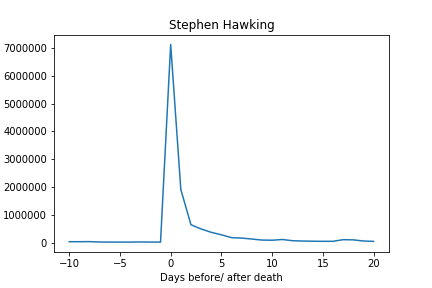
\includegraphics[width=\linewidth]{viewsSH.png}
\endminipage\hfill
\minipage{0.15\textwidth}
  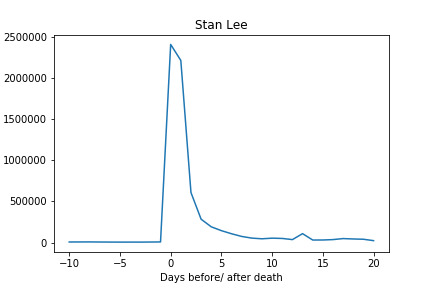
\includegraphics[width=\linewidth]{viewsSL.png}
\endminipage\hfill
\minipage{0.15\textwidth}%
  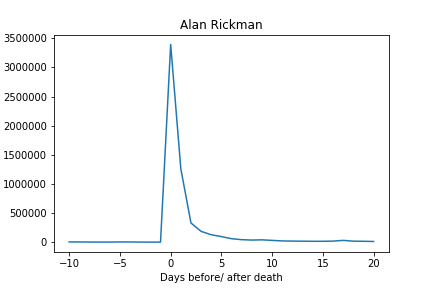
\includegraphics[width=\linewidth]{viewsAR.png}
\endminipage
\caption{Number of views for Stephen Hawking, Stan Lee and Alan Rickman.}
\end{figure}

\subsection{Basic properties}
We start by analysing some basic properties of each graph, such as the number of nodes, the number of edges, the diameter of the (undirected) graph, and the average clustering coefficient (ACC), number of triangles and global clustering coefficient (GCC) with the tools available in Networkx. The results are stated in the  following table. 


\begin{table}[htbp]
\caption{Basic properties of the graphs}
\begin{center}
\begin{tabular}{|c|c|c|c|}
\hline
 Properties & \textbf{Stephen Hawking}& \textbf{Stan Lee}& \textbf{Alan Rickman} \\
\hline
$\#$nodes& & &  \\
\hline
$\#$edges & & &  \\
\hline
Diameter & & &  \\
\hline
ACC& & &  \\
\hline
$\#$triangles  & & &  \\
GCC & & &  \\
\hline
\end{tabular}
\end{center}
\end{table}

\subsection{Degree Distribution}

Here we study the degree distributions of each graph. 

\subsection{Strongly Connected Components}

NOT SURE WE KEEP

\medskip

Our graphs are clearly connected in the undirected sense by the way we have constructed them. In this part we compute the number of strongly connected components. A directed graph is said to be strongly connected if there is a directed path connecting any two of its vertices. 

\subsection{Spectral Clustering }
% Spectral clustering will allow us to see if there are hubs in our graphs. We can use to compare how the signal propagates 

SAME 

\section{Data Exploitation} \label{exploitation}

We now come to the most important part of our analysis, which is the following: we consider the number of views as a signal on the graph. We would like to see how it behaves. In order to make a sensible comparison of number of views and how these number of views evolve for each graph we use the quotient of the number of views before and at the day of the event. 

COMPARE TO RANDOM SIGNAL; HEAT DIFFUSION; ANY OTHER IDEAS? 

\section{Conclusion} \label{conclusion}

Note that if we had the computational power to build a graph with all the pages involved by all the events that we considered together, it would have been much more interesting to see how the number of views evolves locally on the graph. By doing the methods presented in this report, we can only do a “zoom-in” on a specific part of this big graph and analyse it independently of the rest. 


\section*{References}


\cite{laplacian}  
\cite{signalprocessing}
\cite{clustering}

\bibliography{biblio}
\bibliographystyle{plain}

\end{document}
